

\section{時刻同期と測距}

基準となる時刻が違う二つの時間軸を持つ端末間の同期は,互いに音声パルスを出すことで行える(図\ref{fig:beeptobeep}).
この手法はTPSN(time-sync Protocol for sensor network)\cite{tpsn}などで提案されている.
以下で原理について述べる.

\begin{figure}[p]\centering
  \hspace{-2mm}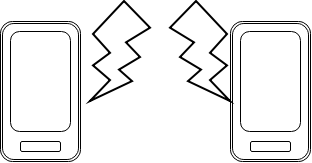
\includegraphics[clip,width=1.1\hsize]{img/beeptobeep.png}
  \caption{2つの端末で互いにパルスを交換する}\label{fig:beeptobeep}
\end{figure}



端末 $A$ が自身の時刻 $t_0$ に音声パルスを発生すると,
そのパルスは音速で空間に広がり,
端末 $B$ 内の時刻 $t_1$ に受信される.
さらに,端末 $B$ からも端末 $B$ 内の時刻 $t_2$ に音声パルスを発すると,
このパルスも音速で空間に広がり,
端末 $A$ 内の時刻 $t_3$ に受信される.
ここで,図\ref{fig:clocksynchronization}の通り,
端末 $A$ 内のパルス時間間隔 $t_3-t_0$ と
端末 $B$ 内のパルス時間間隔 $t_2-t_1$ には差が生じる.

\begin{figure}[p]\centering
  \hspace{-2mm}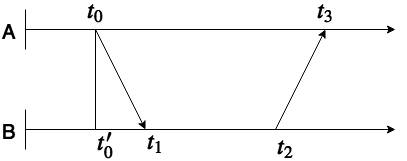
\includegraphics[clip,width=1.1\hsize]{img/clock_synchronization.png}
  \caption{パルス往復時間から伝搬時間を求める}\label{fig:clocksynchronization}
\end{figure}

パルスの往復で伝播にかかった時間は共に等しいと仮定すると,

$$
t_0' = t_1 - \frac{(t_3 - t_0) - (t_2 - t_1)}{2} \\
$$

となり,端末 $B$ 内時刻で端末 $A$ のパルスが発せられた時刻を推定することができる.
以上が時刻同期の原理である.

音速を $c$ とすれば,副次的に端末間の距離も求まる.

$$
d_{AB} = \frac{(t_3 - t_0) - (t_2 - t_1)}{2c}
$$

端末AB間で何らかの処理を同期的に実行したい場合は
図のようにして実行すべき時間を求められる(図\ref{fig:flowchart3}).

\begin{figure}[p]\centering
  \hspace{-2mm}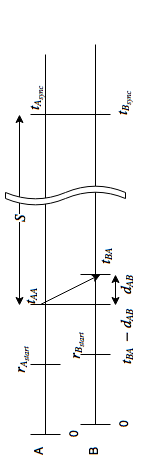
\includegraphics[clip,height=1.5\hsize]{img/flowchart3.png}
  \caption{同期実行方式}\label{fig:flowchart3}
\end{figure}

基準となる端末Aのパルスの受信時間およびその信号の伝達時間と,
それを受信してからの経過時間 $S$ をもとに,同期的に処理を実行できる.

このように,この手法を用いることで,端末間の時刻同期と距離推定を行うことができる.
